\documentclass[10pt,twocolumn,a4paper]{article}

\usepackage{cvpr}
\usepackage{times}
\usepackage{epsfig}
\usepackage{graphicx}
\usepackage{amsmath}
\usepackage{amssymb}
\usepackage{algpseudocode}
\usepackage{multirow}

% Include other packages here, before hyperref.

% If you comment hyperref and then uncomment it, you should delete
% egpaper.aux before re-running latex.  (Or just hit 'q' on the first latex
% run, let it finish, and you should be clear).
\usepackage[breaklinks=true,bookmarks=false]{hyperref}

\cvprfinalcopy % *** Uncomment this line for the final submission

\def\cvprPaperID{****} % *** Enter the CVPR Paper ID here
\def\httilde{\mbox{\tt\raisebox{-.5ex}{\symbol{126}}}}

% Pages are numbered in submission mode, and unnumbered in camera-ready
%\ifcvprfinal\pagestyle{empty}\fi
\setcounter{page}{1}
\begin{document}

%%%%%%%%% TITLE
\title{Perceptron for Predicting Diabetes}

\author{Christopher Hamilton\\
The University of Adelaide\\
{\tt\small christopher.hamilton@student.adelaide.edu.au}
% For a paper whose authors are all at the same institution,
% omit the following lines up until the closing ``}''.
% Additional authors and addresses can be added with ``\and'',
% just like the second author.
% To save space, use either the email address or home page, not both
}

\maketitle
%\thispagestyle{empty}

%%%%%%%%% ABSTRACT
\begin{abstract}
   The is to be in fully-justified italicized text, at the top
   of the left-hand column, below the author and affiliation
   information. Use the word ``Abstract'' as the title, in 12-point
   Times, boldface type, centered relative to the column, initially
   capitalized. The abstract is to be in 10-point, single-spaced type.
   Leave two blank lines after the Abstract, then begin the main text.
   Look at previous CVPR abstracts to get a feel for style and length.
\end{abstract}

%%%%%%%%% BODY TEXT
\section{Introduction}

The prediction of diabetes in individuals without the need for specialised
testing may be beneficial for the early diagnoses of the disease as well
as increasing the number of people who get tested. Given a set of data
relating to a person's health, we may be able to accurately identify
whether or not that individual has diabetes, without the need for a
specific blood test. The set of variables available in the dataset includes
the number of pregnancies, glucose concentration in an oral glucose
concentration test, blood pressure, skin thickness, insulin level, BMI,
diabetes pedigree function and age. These independent variables act as
predictor variables for the single dependent, outcome variable in the
dataset, whether or not the individual has diabetes. As the prediction
is either the individual having diabetes or not, the problem to be solved
is a binary classification problem.

A single perceptron is able to classify data into two classes through linear
separation of the data. The classification is done through the use of a
weighted sum that has a threshold applied and depending on if the sum is
over or under the threshold, the data is classified into either of the classes.

\section{Method}

The perceptron is an adaptive system that is able to recognise patterns in data as well as model the functions of the brain. It was first implemented in 1957 by Frank Rosenblatt at Cornell Aeronautical Laboratory as a way to classify inputs without the need for human action, similar to the human brain. Through research into the physical nervous system and the human brain, discoveries have been made into neuron pathways, and how neurons interact with one another. In humans, it has been discovered that the initial network of connections between neurons is mostly random and as neural activity occurs during development, the reactions of cells to a stimulus changes. Another key result that was found is that when a many stimuli are applied, connections are often formed between the same sets of neurons for similar stimuli and are formed between different sets of neurons for stimuli that are unalike. 

These discoveries have been applied in the development of the perceptron for the binary classification of data. The result of the similar stimuli causing activation for similar neurons has been taken and from this, the perceptron has been designed to classify data to the same class that similar training data was labelled as. A perceptron takes in an input of multiple variables, and based on a set of weights that it has been trained for, generates a weighted sum of these variables. For a perceptron, this weighted sum is used to classify the output into either of the two possible classes, if the sum is greater than or equal to 0, the will be given the positive class (+1) and if it is less than 0, it will be given the negative class (-1).

In order for the perceptron to be able to accurately classify data, it must have weights trained based on a set of inputs which are labelled with correct classes already. The perceptron training algorithm involves setting all weights incorrectly at first, and then iteratively updating the weights based on the product of the training class and the training input data. This algorithm can be written mathematically as:

Assume:
\[ g(\vec{x}; \vec{w}) = sign(\vec{x} \cdot \vec{w}) \]
Where $ \vec{x},\vec{w} \in \mathbb{R}^d $, and $y \in \{-1, 1\} $

For a set of training data: $ \{(\vec{x_i}, y_i)\}_{i=1}^n $,

a step size: $\eta$,

and a number of iterations $T$

The perceptron training algorithm is as follows:
\begin{algorithmic}
\State $\vec{w} \gets \vec{0}$
\For{$t=1$ to $T$}

    $\vec{w_{t+1}} = \vec{w_t} + \eta \sum_{i=1}^n(y_i \vec{x_i} 1_{\{ y_i (\vec{x_i} \cdot \vec{w_t}  ) \leq 0 \}})$
\EndFor
\end{algorithmic}

We denote the trained weights of the perceptron as $w^*$ and this is the same as $w_T$, the weights as updated at the end of the final epoch.

Prediction using this trained perceptron is then done by taking the dot product between the input vector and the weights, to produce a predicted class label, $y^* \in \{-1, 1\}$.

\[ g(\vec{x}; \vec{w^*}) = y^* = sign(\vec{x} \cdot \vec{w^*} ) \]

Since a weighted sum is used as the input to the perceptron, computers are able to very quickly perform the dot products and summations required for the training of a perceptron, as well as the classification of data. This makes the method very useful to quickly classify linearly separable data into one of two classes, given that the weights have been appropriately set to separate the data for the problem to be solved. Setting the weights correctly is the task of the training algorithm that has been outlined above and means that the set of training data points should be large to allow for good generalisation to data points that have not been seen.

The perceptron while able to converge to a prediction for linearly separable data, has some limitations. The first limitation of the perceptron algorithm is that it is only able to converge if the data is linearly separable. This limits the use cases that the perceptron has, a simple example of this is shown in Figure \ref{fig:non-linearly-separable}. Since a lot of data in the real world will not be perfectly linearly separable, the perceptron trained and tested on real data is not likely to have 100\% accuracy. However, this may be acceptable in cases where the perceptron is able to accurately classify test data, even though convergence was not achieved. An example of this is shown in Figure \ref{fig:non-linearly-separable-2}. The data contains two classes, but these cannot be linearly separated, any line drawn to separate the points in this two dimensional space will result in some of the data points being classified incorrectly. In the case of Figure \ref{fig:non-linearly-separable}, the perceptron is not a good solution to classify data points into either of the available classes, as the accuracy will be low. However, in the case of Figure \ref{fig:non-linearly-separable-2}, even though the data is not linearly separable, the perceptron is still an effective method for classifying data points, in the example, only three points are incorrectly labelled based on the linear separation provided.

\begin{figure}
    \centering
    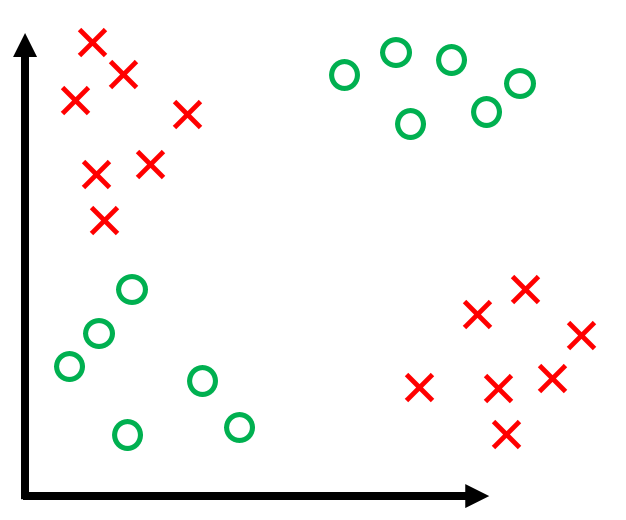
\includegraphics[width=1\linewidth]{non-linearly-separable.png}
    \caption{Example of non-linearly separable data}
    \label{fig:non-linearly-separable}
\end{figure}

\begin{figure}
    \centering
    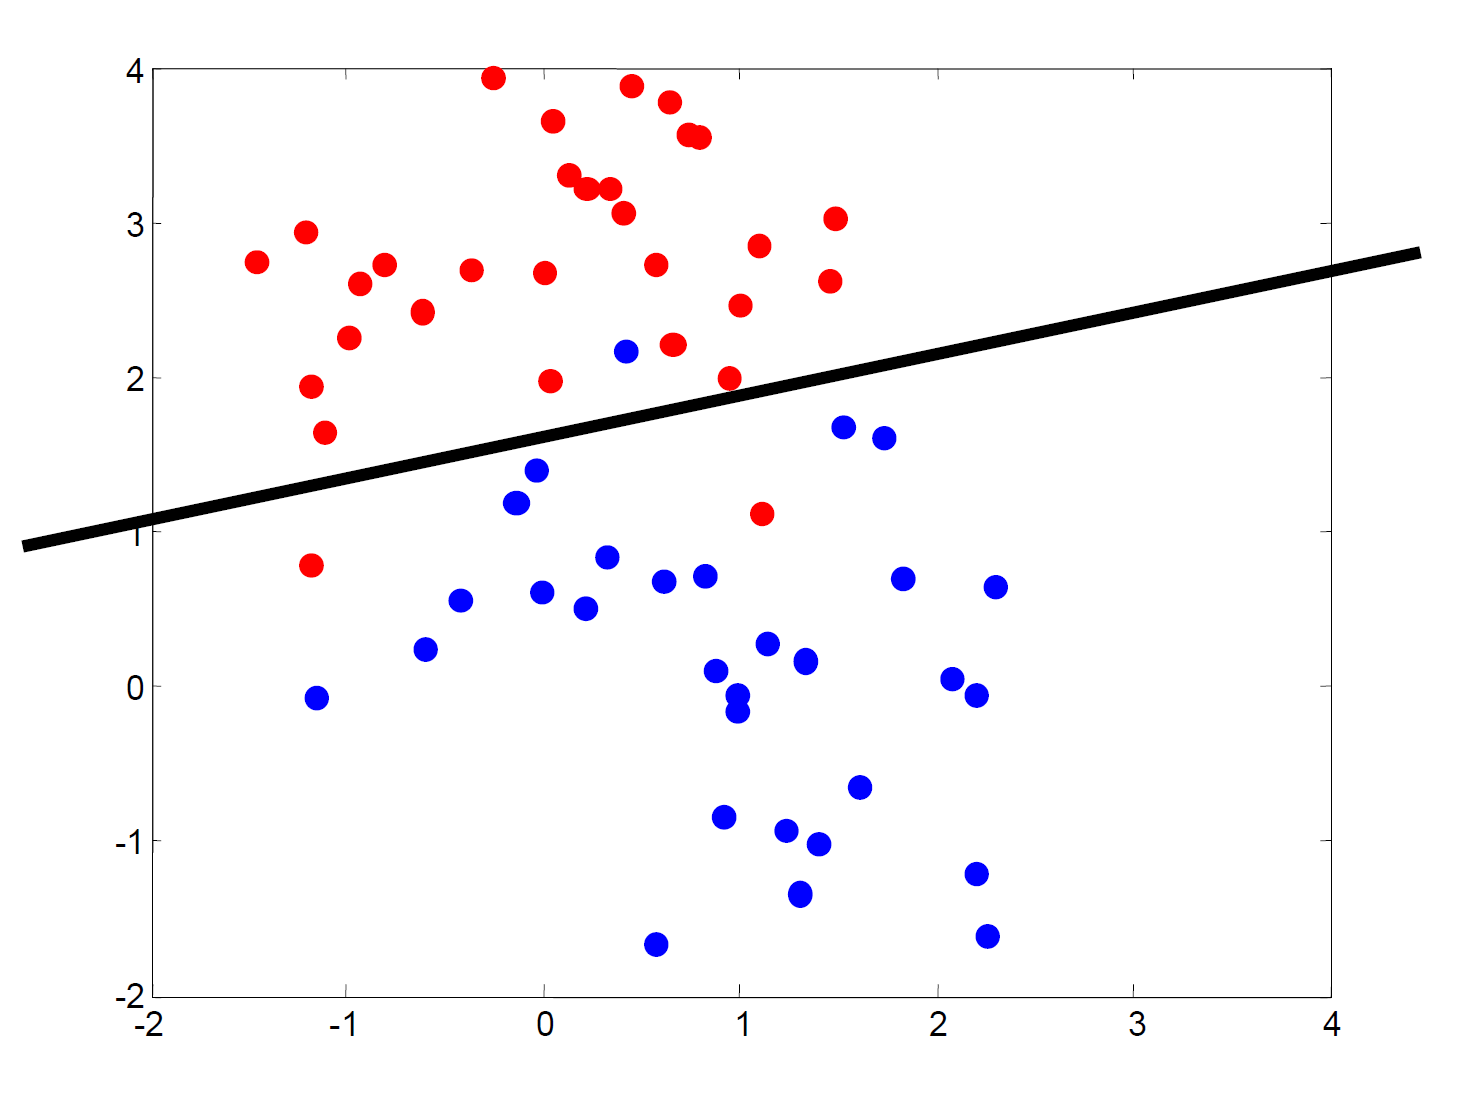
\includegraphics[width=1\linewidth]{non-linearly-separable2.png}
    \caption{Classification of non-linearly separable data TODO: Ref Alexander Ihler https://ics.uci.edu/~kkask/Spring-2018\%20CS273P/slides/05-linClassify.pdf }
    \label{fig:non-linearly-separable-2}
\end{figure}

Another limitation of the perceptron is that it is only able to perform binary classification, and this results in only two options for the predicted class. This works well in data sets where the outcome variable is some sort of indicator variable, however for other use cases, such as data that needs to be classified into three classes, it will not work.

%------------------------------------------------------------------------
\section{Experimental Analysis}

In order to achieve the aim of the experiment, to use a perceptron to predict diabetes, given a set of medical variables, the perceptron algorithm described above in the method section was implemented using Python.  The perceptron needs to have its weights trained in order to produce the separation of the data, and accurately perform predictions. The diabetes data has been pre-processed, with the features being scaled, and the outcome being set to -1 or 1, as required by the perceptron. The diabetes data used can be found at \url{https://www.csie.ntu.edu.tw/~cjlin/libsvmtools/datasets/binary.html}, under the name `diabetes\_scale`. For the purposes of training the perceptron and testing its accuracy, the diabetes data was  randomly split into two sets, one for training and one for testing, with 80\% of data used for training the perceptron and 20% used for testing.

The parameters that can be applied to the training algorithm above are the number of iterations, and the learning rate. In order to determine the optimal learning date and number of iterations, the perceptron should be trained with each set of parameters, and the accuracy should be compared. The values chosen for this are training with 10, 100 and 1000 iterations, as well as 0.1, 0.01 and 0.001 learning rates. The perceptron was run 10 times for each of these sets of values, and the average accuracy produced from predicting the class of test data has been calculated.

\begin{table}[h!]
\begin{center}
\begin{tabular}{ |p{2em}|p{5em}|p{5em}|p{5em}| } 
\hline
Run & Accuracy (\%) $\eta=0.1$ & Accuracy (\%) $\eta=0.01$ & Accuracy (\%) $\eta=0.001$\\
\hline
1 & 33.33 & 54.90 & 52.29 \\
2 & 38.67 & 70.59 & 39.87\\
3 & 69.93	& 62.09 & 58.17 \\
4 & 66.01	& 56.21 & 51.63 \\
5 & 73.86	& 66.01 & 66.01 \\
6 & 71.24	& 40.52 & 69.28 \\
7 & 64.71	& 73.86 & 66.01 \\
8 & 75.16	& 69.93 & 34.64 \\
9 & 74.51	& 50.98 & 71.90 \\
10 & 69.28	& 65.36 & 35.95 \\
\hline
Ave & 63.66	& 61.05 & 54.58 \\
\hline
\end{tabular}
\caption{Results of running experiments with 10 iterations}
\label{table:10iterations}
\end{center}
\end{table}

\begin{table}[h!]
\begin{center}
\begin{tabular}{ |p{2em}|p{5em}|p{5em}|p{5em}| } 
\hline
Run & Accuracy (\%) $\eta=0.1$ & Accuracy (\%) $\eta=0.01$ & Accuracy (\%) $\eta=0.001$\\
\hline
1 & 66.01 & 75.16 & 75.82 \\
2 & 69.93 & 80.39 & 75.82 \\
3 & 66.67 & 66.67 & 71.90 \\
4& 67.97 & 77.78 & 64.71 \\
5& 58.82 & 55.56 & 72.55 \\
6& 56.21 & 73.20 & 60.13 \\
7& 75.16 & 70.59 & 79.08 \\
8& 62.75 & 66.01 & 70.59 \\
9& 78.43 & 72.55 & 69.28 \\
10& 67.97 & 75.16 & 68.63 \\
\hline
Ave& 66.99 & 71.31 & 70.85 \\

\hline
\end{tabular}
\caption{Results of running experiments with 100 iterations}
\label{table:100iterations}
\end{center}
\end{table}

\begin{table}[h!]
\begin{center}
\begin{tabular}{ |p{2em}|p{5em}|p{5em}|p{5em}| } 
\hline
Run & Accuracy (\%) $\eta=0.1$ & Accuracy (\%) $\eta=0.01$ & Accuracy (\%) $\eta=0.001$\\
\hline
1& 69.28& 67.97& 71.90 \\
2& 63.40& 71.90& 64.05 \\
3& 64.71& 64.71& 71.24 \\
4& 58.82& 77.12& 64.71 \\
5& 75.16& 79.08& 70.59 \\
6& 66.67& 55.56& 64.71 \\
7& 63.40& 66.67& 64.71 \\
8& 74.51& 66.01& 73.86 \\
9& 75.82& 65.36& 70.59 \\
10& 74.51& 67.97& 59.48 \\
\hline
Ave& 68.63& 68.24& 67.58 \\

\hline
\end{tabular}
\caption{Results of running experiments with 1000 iterations}
\label{table:1000iterations}
\end{center}
\end{table}

After running the code multiple times, it can be observed that the accuracy produced can be quite varied between a run. This implies that the data is likely not linearly separable, and since the weights are not able to converge, not all data points can be classified correctly. However, taking an average may be able to give a better representation of the accuracy for a given learning rate and number of iterations.

Based on the results seen in Table \ref{table:10iterations}, Table \ref{table:100iterations}, and Table \ref{table:1000iterations}, the highest accuracy was achieved using a learning rate of eta = 0.01 and training for 100 iterations. For the experiments where training was only done for 10 iterations, the accuracy on average was lower for all learning rates, however, it can be noted that for less iterations, a higher learning rate was more effective in producing a higher accuracy model. For experiments done with 1000 iterations, it can be seen that the accuracy is very close to the highest accuracy produced, and that the learning rate has only a small effect on the average accuracy. This is likely because after this larger number of iterations, the model will reach similar weights, regardless of the learning rate used.


%------------------------------------------------------------------------
\section{Code}

The code written to implement the perceptron algorithm can be found at \url{https://github.com/CHamilton0/COMP-SCI-7318-Deep-Learning-Fundametals}. It has been implemented in Python 3.11.9. From the Assignment1 directory in the above repository. To load the diabetes data, run the perceptron training algorithm and run predictions on the data, ensure numpy is installed with python3 -m pip install numpy and then run the code with python3 perceptron.py. A helper script has been written in order to load the diabetes data in a form that the perceptron can work with. This loading function has been implemented in the `load\_diabetes.py` script. It will open the diabetes data file, and split the data in each line into the vector of variables and the outcome. These tuples of inputs and outcomes are then shuffled to randomise the data that is used for training and testing. In investigating the training and testing data, it was found that some rows in the data do not have all the variables set, for rows where not all variables are set, the script to load the data will leave the unset value as zero in the input vector, this will result in it not having an effect on the dot product done as part of training or classification. 

The perceptron.py script contains the implementation of the perceptron algorithm used. Weights are initialised to zero, and are updated for the training data that the perceptron has classified incorrectly. This is repeated for the number of iterations specified by T. Finally, the test data is classified with the trained perceptron, as described in the algorithm, and checked against the label. The accuracy, as a percentage of correct classifications on the test data, is calculated and displayed in the terminal.

%------------------------------------------------------------------------

{\small
\bibliographystyle{ieee_fullname}
\bibliography{egbib}
}

\end{document}
